%!TEX root = Slides.tex
\part{Einf\"uhrung in das Datenbankkonzept}
\label{part:grundlagen}
\pdfbookmark[-1]{Grundlagen}{grundlagen}

\section{Motivation und Einführung}

\subsection{Grundlagen und Anforderungen}

\begin{frame}{\insertsection}
	\framesubtitle{\insertsubsection}
	\begin{alertblock}{\Large Kurze Diskussionsrunde}
	\begin{center}
		\Large{Was ist eine Datenbank?}
	\end{center}		
	\end{alertblock}
\end{frame}

\begin{frame}{\insertsection}
\framesubtitle{\insertsubsection}
\structure{Anwendungssysteme arbeiten auf Daten.}
\begin{itemize}
	\item Buchungs- oder Bibliothekssysteme, ERP-Systeme etc.
	\item Multimediadatenbanken
	\item Geoinformationssysteme
	\item Zeitreihendatenbanken
\end{itemize}
\onslide\pause
\abs 
\structure{Basisoperationen (CRUD-Operationen)}
\begin{itemize}
	\item Erzeugen (Create)
	\item Lesen (Read)
	\item Verändern (Update)
	\item Löschen (Delete)
\end{itemize}
\end{frame}

\subsection{Historische Einordnung}

\begin{frame}{\insertsection}
\framesubtitle{\insertsubsection}
\structure{50er Jahre}
	\begin{figure}
	\pgfuseimage{lochkarte} \hspace{2em}
	\pgfuseimage{magnetband}
	\caption{Lochkarte und Magnetband}
	\end{figure}
		\begin{itemize}
			\item Zugriff auf die Medien war nur sequentiell möglich
			\item Mechanische Verschleißerscheinungen / generelle Empfindlichkeit der Medien
			\item Lange Zugriffszeiten
			\item Fassungsvermögen einer Lochkarte: Zwischen $60-100$ Bytes
		\end{itemize}
\end{frame}

%\begin{frame}{Die 50er Jahre}
%\framesubtitle{Lochkarten und Magnetbänder}
%
%\begin{block}{Rechenbeispiel anhand der Wikipedia-Datenmenge (44GB, Stand 2013)}
%	\begin{itemize}
%		\item Voraussichtliche Menge der benötigten Lochkarten: $5.9 \cdot 10^8$
%		\item Höhe des Lochkartenstapels: ca. $100$km
%		\item Gesamtgewicht: $1450$t
%		\item Längs aneinandergelegt könnte man 17x die Erde umrunden.
%	\end{itemize}
%\end{block}
%\end{frame}

\begin{frame}{\insertsection}
	\framesubtitle{\insertsubsection}
	\structure{60er und 70er Jahre: Festplatten}
		\begin{itemize}
			\item Datenspeicherung in logischen Einheiten (Dateien)
			\item Direkte, nicht-sequentielle Adressierung
			\item Mittlere Zugriffszeit nur noch Sekundenbruchteile
			\item Datenmanipulation wesentlich einfacher
		\end{itemize}

	\begin{columns}
		\begin{column}{.48\textwidth}
			\begin{tabbing}
				\texttt{Schmidt   } \= \texttt{Heiko   } \= \texttt{1948} \kill
				\textbf{Fixlängendatei} \> \> \\
				\texttt{Schmidt} \> \texttt{Heiko} \> \texttt{1948} \\
				\texttt{Zander} \> \texttt{Uwe} \> \texttt{2011}
			\end{tabbing}
		\end{column}

		\begin{column}{.48\textwidth}
			\begin{tabbing}
				\texttt{Placeholder} \= \kill
				\textbf{CSV-Datei}\\
				\texttt{Schmidt;Heiko;1948}\\
				\texttt{Zander;Uwe;2011}
			\end{tabbing}
		\end{column}
	\end{columns}

	\onslide\pause 
	\begin{alertblock}{Frage}
	Welche datenbezogenen Funktionen muss eine dateibasierte Anwendung zur Speicherung von Kunden- und 
	Auftragsdaten eines größeren Unternehmens beinhalten? Wie würden Sie diese implementieren? Skizzieren 
	Sie die Funktionen/Methoden.
	\end{alertblock}
	
\end{frame}

\subsection{Dateibasierte Datenhaltung}

\begin{frame}{\insertsection}
	\framesubtitle{\insertsubsection}
	\structure{Konkurrierender Zugriff}
	\begin{columns}
		\begin{column}{.40\textwidth}
			\begin{figure}
				\pgfuseimage{concurrentAccess}
			\end{figure}
		\end{column}
		\begin{column}{.56\textwidth}
			\begin{itemize}
				\item Datei unter Kontrolle des Betriebssystems: Shared und Exclusive Locks auf Dateiebene
				\item \alert{Potentielle Gefahr inkonsistenter Daten!}
			\end{itemize}
		\end{column}
	\end{columns}
\end{frame}

\begin{frame}{\insertsection}
	\framesubtitle{\insertsubsection}
	\structure{Zusammenfassung der Problemstellung}
	 \begin{itemize}
		\item Redundanz und Inkonsistenz
		\item Beschränkte Zugriffsmöglichkeiten
		\item Probleme im Mehrbenutzerbetrieb
		\item Verlust von Daten im Fehlerfall
		\item Integritätsverletzung
		\item Sicherheitsprobleme
		\item Hohe Entwicklungskosten
	\end{itemize}

	\alert{$\Rightarrow$ Dem Datei-Ansatz mangelt es an der nötigen Flexibilität}
\end{frame}

\subsection{Grundidee des Datenbankkonzeptes}

\begin{frame}[t]{\insertsection}
\framesubtitle{\insertsubsection}
\begin{block}{Anforderungen an eine moderne Datenhaltung}
	\begin{itemize}
		\item Skalierbarkeit
		\item Performanz auch bei großen Datenmengen
		\item Sicherstellung der Datenintegrität
		\item Ermöglichung konkurrierender Zugriffe
		\item Strukturelle Änderungen müssen einfach zu realisieren sein
		\item Datenschutz vor unberechtigten Zugriffen
	\end{itemize}
\end{block}
%\abs 
%\structure{ Diese Anforderungen waren nicht immer selbstverständlich!}
\end{frame}

\begin{frame}{\insertsection}
	\framesubtitle{\insertsubsection}
	\begin{itemize}
		\item Daten werden anhand eines vorher festgelegten \textit{Schemas} gespeichert
		\begin{itemize}
			\item Was für Daten?
			\item Welche Einschränkungen?
			\item Beziehungen untereinander?
		\end{itemize}
		\item Es werden Daten \textit{und} Schema in der Datenbank gespeichert
		\item Die Integrität wird erzwungen
		\item Daten werden von Anwendungen getrennt
		\item Unterschiedlichen Benutzern können \textit{Sichten} auf die Daten bereitgestellt werden
		\item Konkurrierende Zugriffe von zentraler Instanz koordiniert
	\end{itemize}
\end{frame}

\begin{frame}{\insertsection}
\framesubtitle{\insertsubsection}
\begin{columns}
	\begin{column}{.35\textwidth}
		\begin{figure}
			\begin{tikzpicture}
			\filldraw[drop shadow, black!20] (0,0.3) rectangle (4,4.7);
			\node at (2.0,4.4) {DBS};
			\filldraw[drop shadow, yellow] (0.5,0.5) rectangle (3.5,4.0);
			\node at (2.0,3.7) {DBMS};			
			\filldraw[drop shadow, green] (0.8,0.7) rectangle (3.2,3.4);
			\node at (2.0,3.15) {DB};
			\node at (2,2.3) [drop shadow, fill=orange, cylinder,minimum height=1cm, draw, shape border rotate=90, minimum width=2cm] {};
			\node at (2,2.4) {Datenbasis};
			\node at (2,1.2) [drop shadow, fill=orange, cylinder,minimum height=1cm, draw, shape border rotate=90, minimum width=2cm] {};
			\node at (2,1.2) {Metadaten};
			\end{tikzpicture}
			\caption{Datenbankkonzept}
		\end{figure}
	\end{column}
	
	\begin{column}{.6\textwidth}
		\begin{description}
			\item[DBS:] Datenbanksystem
			\item[DBMS:] Datenbankmanagementsystem
			\item[DB:] Bestehend aus Datenbasis (Nutzdaten) und Metadaten (Daten über Daten)
		\end{description}
		\onslide
		\pause
		\begin{itemize} 
			\item Datenbank(en) werden durch DBMS verwaltet.
			\item Anwendungen greifen über das DBMS auf die Daten der Datenbank(en) zu. 
		\end{itemize} 
	\end{column}
\end{columns}
\end{frame}

\section{Grundlagen}
\subsection{Terminologie}



\begin{frame}{\insertsection}
	\framesubtitle{\insertsubsection}
	\begin{definition}[Datenbank]
		Eine Datenbank ist eine Sammlung von Daten, die einen Ausschnitt der realen Welt beschreiben. Unter Daten verstehen 
		wir bekannte Tatsachen, die aufgezeichnet werden können und eine implizite Bedeutung haben  (vgl. \cite[S. 4]{EN10}).
	\end{definition}
  \abs\onslide\pause
	\structure{Eigenschaften von Datenbanken:}
	\begin{itemize}
		\item Eine Datenbank stellt Aspekte der realen Welt (Universe of Discourse) dar. Änderungen im Universe of Discourse spiegeln sich in der Datenbank.
		\item Eine Datenbank ist eine logisch zusammenhängende Sammlung von Daten mit einer \textbf{inhärenten Bedeutung}.
		\item Eine Datenbank wird für einen bestimmten Zweck entworfen, entwickelt und mit Daten gefüllt.
	\end{itemize}
\end{frame}


\begin{frame}{\insertsection}
	\framesubtitle{\insertsubsection}
	\begin{definition}[Datenbankmanagementsystem]
		Ein Datenbankmanagementsystem (DBMS) ist ein Softwaresystem, welches dem Benutzer das Erstellen und die Pflege von Datenbanken 
		erm\"oglicht und Benutzern oder Anwendungen den Zugriff auf die Datenbanken \"uber Datenbankanfragen gew\"ahrt 
		(vgl. \cite[S. 5]{EN10}).
	\end{definition}
  \abs\onslide\pause 
	\structure{Verantwortlichkeiten}
	\begin{enumerate}
		\item Definition der Daten: Spezifikationen von Datentypen, Strukturen und Einschränkungen $\Rightarrow$ Metadaten
		\item Konstruktion der Daten: Speichern der Daten auf ein physisches Medium 
		(wird hier nicht weiter betrachtet $\Rightarrow$ Vorlesung \textit{Datenbanktechnik})
		\item Manipulation der Daten: CRUD-Operationen
	\end{enumerate}	
\end{frame}

%\begin{frame}{\insertsection}
%	\framesubtitle{\insertsubsection}
%	\begin{definition}[Datenbankmanagementsystem]
%		Ein Datenbankmanagementsystem ist ein Softwaresystem, welches dem Benutzer das Erstellen und die Pflege einer Datenbank ermöglicht  (vgl. \cite[S. 5]{EN10}).
%	\end{definition}
	
%	\structure{Verantwortlichkeiten  (vgl. \cite[S. 5]{EN10})}
%	\begin{enumerate}
%		\item Definition der Daten: Spezifikationen von Datentypen, Strukturen und Einschränkungen
%		\item Konstruktion der Daten: Speichern der Daten auf ein physisches Medium (wird hier nicht weiter betrachtet: $\Rightarrow$ Vorlesung \textit{Datenbanktechnik})
%		\item Manipulation der Daten: CRUD-Operationen
%	\end{enumerate}
	
%	\vspace{2em}
%	Applikationen greifen auf die Datenbank zu, indem sie Anfragen an das DBMS schicken. 
%\end{frame}

\subsection{Datenabstraktion und ANSI/SPARC-Modell}

\begin{frame}[label=ansisparc]{\insertsection}
\framesubtitle{\insertsubsection}

	\begin{columns}
		\begin{column}{.48\textwidth}
			\begin{figure}
				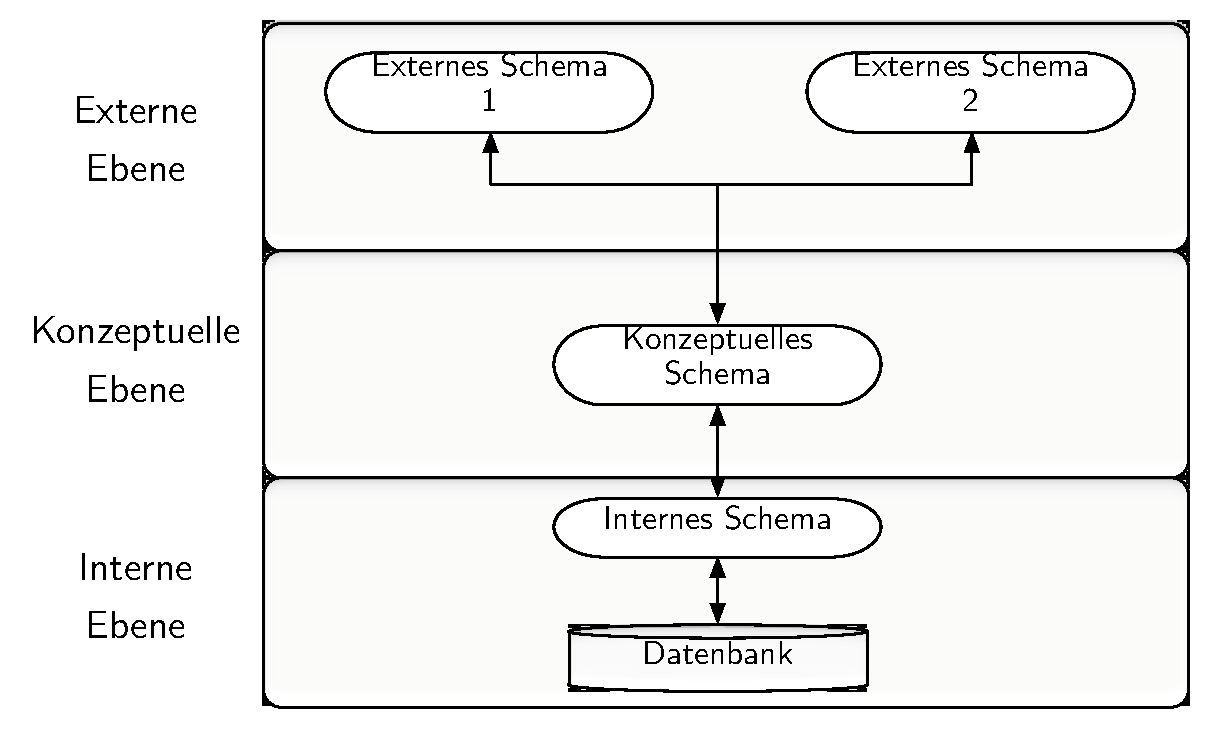
\includegraphics[scale=0.35]{img/ansisparc.pdf}
			\end{figure}
		\end{column}
		\begin{column}{.48\textwidth}
		\structure{ANSI/SPARC 3-Schicht-Architektur}
			\begin{itemize}
				\item Externe Ebene beschreibt Sichten auf die Daten
				\item Konzeptuelle Ebene beschreibt die system- und anwendungsunabhängige Struktur
				\item Interne Ebene beschreibt physische Speicherstrukturen einer Datenbank
			\end{itemize}
			\structure{Gewährleistung der logischen und physischen Datenunabhängigkeit}
		\end{column}
	\end{columns}
\end{frame}

\begin{frame}{\insertsection}
	\framesubtitle{\insertsubsection}
	\begin{block}{Physische Datenunabhängigkeit}
		\begin{itemize}
			\item Physische Speicherstrukturen werden verborgen
			\item Änderungen an der physischen Struktur haben keinen Einfluss auf die konzeptuelle Struktur
		\end{itemize}
	\end{block}

	\begin{block}{Logische Datenunabhängigkeit}
		\begin{itemize}
			\item Konzeptuelle Strukturen werden verdeckt
			\item Zugriff auf Daten über Sichten
			\item Änderungen an konzeptueller Struktur haben keinen Einfluss auf die Sichten
		\end{itemize}
	\end{block}
	\alert{Die logische Datenunabhängigkeit ist wesentlich schwerer zu erreichen als die physische und kann nur für einfachste 
		Modifikationen des Datenbankschemas gewährleistet werden!}
\end{frame}

\subsection{Generelle Architektur eines DBMS}
\begin{frame}{\insertsection}
	\framesubtitle{\insertsubsection}

	\begin{figure}
		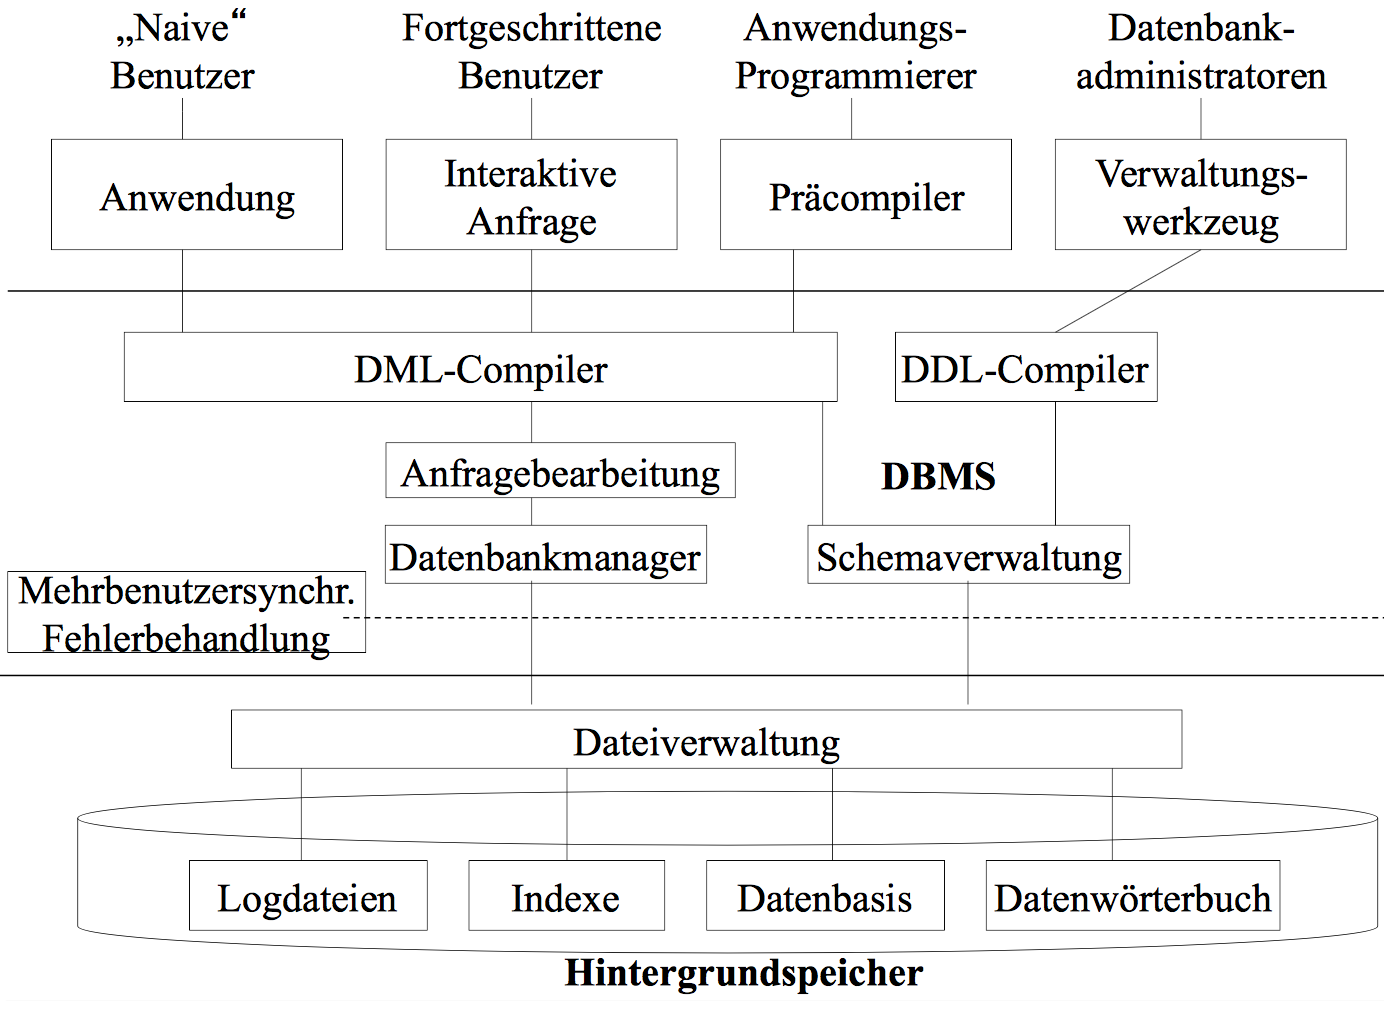
\includegraphics[scale=0.16]{img/db_arch.png}
		\caption{Architekturübersicht eines DBMS (vgl. \cite[S. 31]{KE15})}
	\end{figure}
\end{frame}

\begin{frame}{\insertsection}
	\framesubtitle{\insertsubsection}
	\structure{Vorteile bei der Nutzung eines DBMS:}
	\begin{itemize}
		\item Kontrolle über Redundanzen 
		\item Zugriffskontrolle der Benutzer \"uber Authentisierung und Autorisierung
		\item Persistenter Datenspeicher für Programmobjekte 
		\item Realisierung von Speicherstrukturen und effizienten Suchtechniken 
		\item Backup und Recovery 
		\item Ermöglichen eine Vielzahl von Benutzerschnittstellen 
		\item Repräsentieren komplexe Beziehungen entlang der Daten 
		\item Sicherstellung der referentiellen Integrität		
	\end{itemize}
	
\end{frame}

\section*{Übungsaufgaben}
%\subsection*{Grundlegendes Datenbankverständnis}
\begin{frame}{\insertsection}
	%\framesubtitle{\insertsubsection}
\begin{alertblock}{Grundlegendes Datenbankverständnis}
	\begin{enumerate}
		\item Benennen Sie die Problemstellungen dateibasierter Datenhaltung in einem Dateisystem. Erläutern Sie auch die Schwierigkeiten, die bei der Entwicklung dateibasierter Anwendungen existieren.
		\item Grenzen Sie die Begriffe \textit{Datenbank} und \textit{Datenbankmanagementsystem} voneinander ab.
		\item Erläutern Sie das ANSI/SPARC-Modell sowie die Begriffe \textit{logische} und \textit{physische} Datenunabhängigkeit.
		\item Beschreiben Sie die Vorteile beim Einsatz eines DBMS jeweils anhand eines Beispiels.
		\item Können Sie sich nachteilige Eigenschaften eines DBMS vorstellen, sodass ein DBMS in bestimmten Szenarien \textit{keinen} Einsatz finden sollte?
		\item Erläutern Sie die Komponenten der Datenbankarchitektur.
	\end{enumerate}
	\end{alertblock}
\end{frame}

%\section*{Zusammenfassung}
%\begin{frame}{Zusammenfassung}
%	\begin{itemize}
%		\item Anforderungen von Applikationen an die Datenhaltung
%		\item Historische Einordnung
%		\item Erläuterung der Problemstellungen dateibasierter Datenhaltung
%		\item Terminologien
%		\begin{itemize}
%			\item Datenbank und Datenbankmanagementsystem
%			\item Datenmodelle, Schemata und Datenbankzustand
%		\end{itemize}
%		\item ANSI/SPARC Architekturmodell
%		\item Datenbanksprachen
%		\item Beteiligte Akteure
%	\end{itemize}
%\end{frame}
